\subsection{Ausgabeknoten}

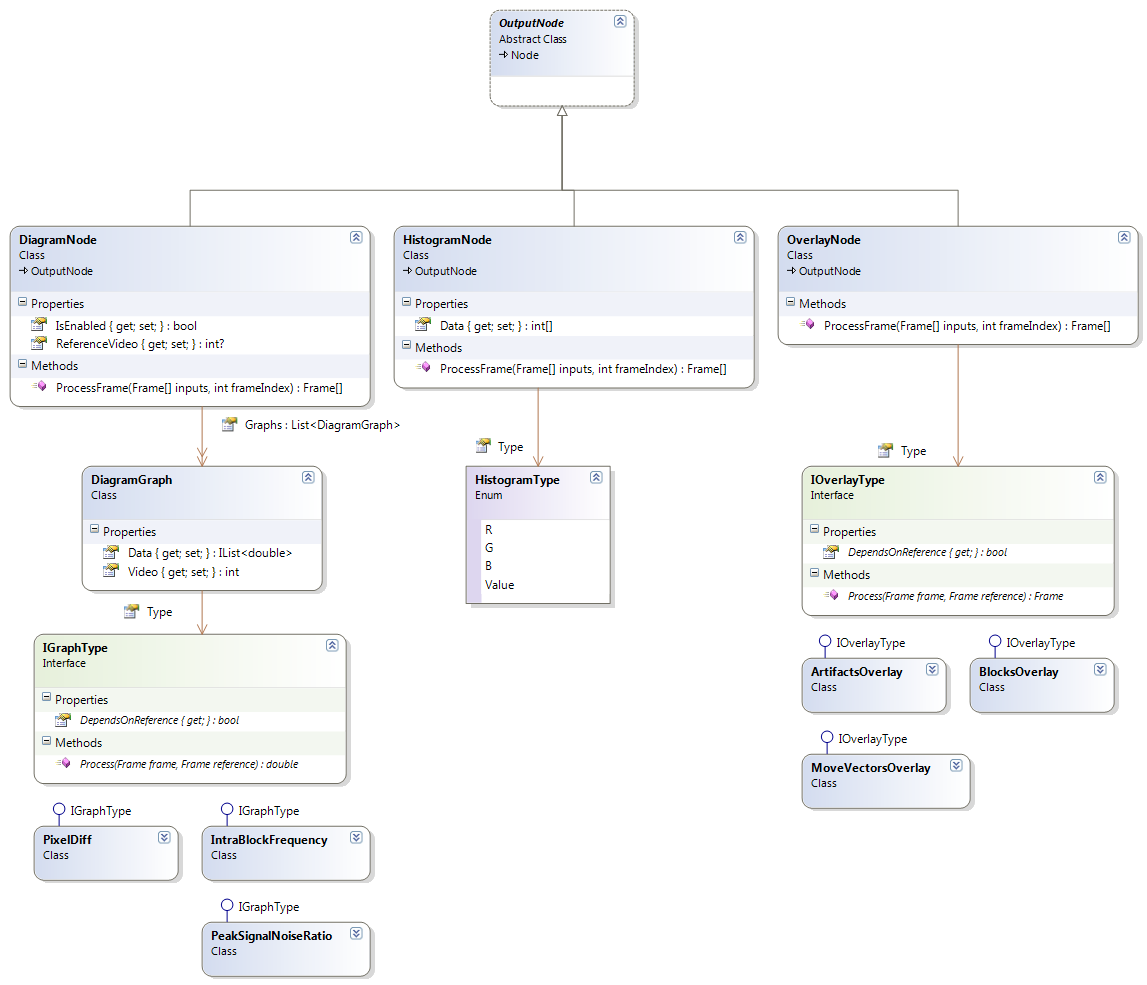
\includegraphics[width=\textwidth]{YuvKA.Pipeline/outputnodes.png}
UML-Klassendiagramm der Knoten, die für die Wiedergabe, Analyse und Vergleich von Videos in der Pipeline zuständig sind.

\subsubsection{YuvKA.Pipeline.Outputnode}

\begin{verbatim}
public abstract class OutputNode : Node
\end{verbatim}

\paragraph{Beschreibung}~\\
Die abstrakte Klasse \name{OutputNode} modelliert die Ausgabemöglichkeiten der Pipeline und bietet eine gemeinsame Basis für deren konkrete Implementationen.

\subsubsection{YuvKA.Pipeline.DiagrammNode}

\subsubsection{YuvKA.Pipeline.HistogramNode}

\subsubsection{YuvKA.Pipeline.OverlayNode}

\begin{verbatim}
public class OverlayNode : OutputNode
\end{verbatim}

\paragraph{Beschreibung}~\\
Die Klasse \name{OverlayNode} modelliert das Überlagern von Videos mit graphischen Darstellungen von Analysedaten.

\paragraph{Typmember}
\begin{itemize}

\property{Type}
	\begin{verbatim}
	public IOverlayType Type { get; set; }
	\end{verbatim}
	Ruft die Art der Überlagerung ab, oder legt sie fest. Standardmäßig werden die Markierung von Artefakten im Vergleich mit einem Referenzvideo, das Anzeigen von Bewegungsvektoren sowie eine Anzeige der Makroblockentscheidungen des Encoders unterstützt.

\method{ProcessFrame}
	\begin{verbatim}
	public override Frame[] ProcessFrame(Frame[] inputs, int frameIndex)
	\end{verbatim}
	Überlagert den übergebenen \name{Frame} mit den durch \name{Type} spezifizierten Daten und gibt den Überlagerten \name{Frame} zurück. Bei den standardmäßig unterstützen Möglichkeiten handelt es sich um:
	\begin{description}
		\item[Artefaktüberlagerung]~\\
			Für diese Überlagerung werden zwei Eingabeframes benötigt, da hier die Artefakte eines \name{Frame}s im Vergleich mit einem anderen hervorgehoben werden.
		\item[Blocküberlagerung]~\\
			Für diese Überlagerung wird eine Eingabe in Form eines \name{AnnotatedFrame}s benötigt, da aus den Logdateien die Makroblockentscheidungen des Encoders entnommen werden um damit die Darstellung dieser Entscheidungen über dem \name{Frame} zu legen.
		\item[MoveVectorsOverlay]~\\
			Für diese Überlagerung wird eine Eingabe in Form eines \name{AnnotatedFrame}s benötigt, da aus den Logdateien die erkannten Bewegungsvektoren des Encoders entnommen werden um diese in den \name{Frame} einzuzeichnen.
	\end{description}
	
\end{itemize}